\subsection{\textbf{Giroscopio}:}	
El giroscopio es un sensor que mide la velocidad angular o la tasa de rotación de un objeto alrededor de tres ejes perpendiculares entre sí: X, Y y Z. Su función principal es detectar cambios en la orientación de un objeto y mantener la estabilidad en sistemas en movimiento. Los giroscopios se basan en principios físicos, como el efecto giroscópico, para proporcionar mediciones precisas y estables de rotación.


Aplicaciones en Robótica:


Los giroscopios son esenciales en la navegación de robots móviles, particularmente en sistemas que requieren un control preciso de su orientación. Al integrarse con otros sensores como el acelerómetro y el magnetómetro, el giroscopio permite a los robots mantener la estabilidad y orientación durante el movimiento. En la robótica avanzada, esto es crucial para robots autónomos que deben operar en entornos complejos, donde las variaciones en el terreno y las posibles interferencias en la señal del GPS pueden afectar la capacidad de navegación. Sin un giroscopio, los robots tendrían dificultades para realizar tareas como el balanceo, el vuelo o la navegación precisa en entornos 3D, lo que afectaría su autonomía y fiabilidad.


Impacto en la Robótica Avanzada:


En robótica avanzada, los giroscopios permiten a los robots realizar movimientos más fluidos y controlados, lo que es esencial para tareas que requieren alta precisión, como la manipulación de objetos delicados, el vuelo de drones o la navegación en terrenos irregulares. Además, al integrarse en sistemas de control de actitud, ayudan a los robots a mantener una posición y orientación constantes, incluso cuando experimentan perturbaciones externas, como vientos o colisiones ligeras.

Según \cite{grewal2014kalman} asi esta definido el giroscopio.

\begin{figure} [h]
	\centering
	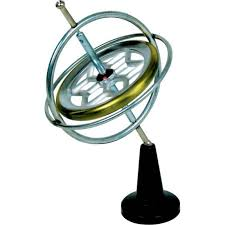
\includegraphics[width=0.2\linewidth]{img/giroscopio}
	\caption{}
	\label{fig:giroscopio}
\end{figure}

\subsection{\textbf{Acelerometro}:}

El acelerómetro es un sensor que mide la aceleración a lo largo de tres ejes perpendiculares entre sí: X, Y y Z. Este dispositivo detecta cambios en la velocidad de un objeto y la aceleración debida a la gravedad, lo que le permite calcular la velocidad y la posición de un objeto en movimiento. Además, los acelerómetros pueden detectar vibraciones y movimientos sutiles en un sistema, lo que los hace útiles para tareas que requieren monitorización precisa de la dinámica de los objetos.


Aplicaciones en Robótica:


En robótica, los acelerómetros se utilizan principalmente para monitorear y ajustar el movimiento y la postura de los robots. Estos sensores son críticos para la estabilización y control de robots móviles, como los vehículos autónomos y los drones. Los robots que deben moverse en terrenos irregulares o navegar a través de espacios confinados se benefician enormemente de los acelerómetros, ya que estos sensores les permiten ajustar su comportamiento en respuesta a la aceleración y las fuerzas gravitacionales. Asimismo, en aplicaciones de robótica humana, como los exoesqueletos o los dispositivos de asistencia, los acelerómetros proporcionan información clave para ajustar los movimientos del robot y garantizar la seguridad y comodidad del usuario.


Impacto en la Robótica Avanzada:


La integración de acelerómetros en sistemas robóticos avanzados permite la navegación precisa, el control del balance y la detección de caídas o desequilibrios. En robots de servicio, drones y vehículos autónomos, la capacidad de detectar movimientos rápidos y ajustes sutiles en la aceleración mejora la estabilidad y la precisión operativa. Además, la información proporcionada por el acelerómetro es crucial para la simulación del comportamiento dinámico de un robot, permitiendo una interacción más eficiente con su entorno.

Según \cite{kuo2017automatic} asi esta definido el acelerometro.

\begin{figure} [h]
	\centering
	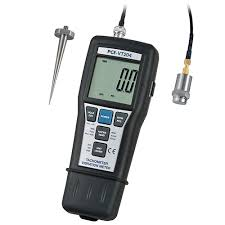
\includegraphics[width=0.3\linewidth]{img/acelerometro}
	\caption{}
	\label{fig:acelerometro}
\end{figure}
\subsection{\textbf{Magnetómetro}:}

El magnetómetro es un sensor que mide la intensidad y dirección del campo magnético terrestre. Este sensor permite determinar la orientación absoluta de un robot en relación con el norte magnético, lo que es especialmente útil para mejorar la precisión en la navegación en entornos desconocidos. Al ser sensible a las variaciones en el campo magnético terrestre, los magnetómetros son una herramienta clave para complementar la información proporcionada por otros sensores, como el giroscopio y el acelerómetro.



Aplicaciones en Robótica:


Los magnetómetros son particularmente valiosos en la navegación de robots en entornos GPS-denegados, como túneles, edificios o áreas subterráneas. Al proporcionar información adicional sobre la orientación en relación con el norte magnético, los magnetómetros permiten a los robots mantener una ruta de navegación precisa, incluso cuando otras fuentes de información, como los sistemas GPS, no están disponibles. Este tipo de sensor es crucial en aplicaciones donde se requiere una orientación constante, como en la navegación submarina o en misiones de exploración planetaria.


Impacto en la Robótica Avanzada:


En la robótica avanzada, los magnetómetros mejoran significativamente la capacidad de los robots para navegar con precisión en entornos complejos. Al integrar este sensor con otros, como el giroscopio y el acelerómetro, los robots pueden realizar correcciones más precisas en su ruta y mantener una orientación adecuada en condiciones difíciles. Esto es esencial en aplicaciones como la exploración autónoma de terrenos desconocidos o el control preciso de robots en espacios sin referencias externas.

Según \cite{park2017design} esta es la definicion de magnetómetro.
\begin{figure}[h]
	\centering
	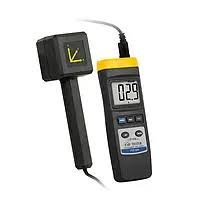
\includegraphics[width=0.3\linewidth]{img/magnetometro}
	\caption{}
	\label{fig:magnetometro}
\end{figure}
\subsection{ \textbf{LiDAR (Light Detection and Ranging}):}

LiDAR es una tecnología de detección remota que utiliza pulsos láser para medir distancias y crear mapas tridimensionales detallados del entorno. Emite pulsos de luz láser y mide el tiempo que tarda cada pulso en reflejarse de vuelta al sensor, calculando así la distancia a los objetos en su campo de visión. Los sistemas LiDAR son extremadamente precisos y pueden crear mapas detallados en tiempo real. \cite{wehr1999airborne}.


Aplicaciones en Robótica:


En la robótica avanzada, LiDAR se utiliza para crear representaciones tridimensionales del entorno, lo que facilita la navegación autónoma y la detección de obstáculos. Los robots equipados con LiDAR pueden mapear su entorno con alta precisión, lo que les permite detectar y evitar obstáculos, reconocer objetos y realizar tareas como el escaneo y análisis de terrenos. Además, LiDAR se utiliza en vehículos autónomos para realizar mapas precisos de la carretera y el entorno circundante, asegurando una conducción segura y eficiente.


Impacto en la Robótica Avanzada:


LiDAR ha transformado la robótica avanzada al proporcionar una capacidad sin precedentes para mapear y navegar de manera autónoma en entornos complejos y dinámicos. Gracias a su alta resolución y precisión, LiDAR es un componente fundamental en aplicaciones de robótica que requieren una navegación avanzada, como vehículos autónomos, drones de mapeo y robots de inspección en lugares peligrosos o inaccesibles. Esta tecnología permite a los robots tomar decisiones informadas sobre su entorno y ajustar sus acciones en consecuencia, lo que mejora la eficiencia y la seguridad.
\begin{figure} [h]
	\centering
	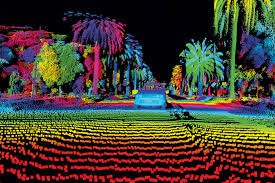
\includegraphics[width=0.3\linewidth]{img/lidar}
	\caption{}
	\label{fig:lidar}
\end{figure}

\newpage
\subsection{Clasificación de Sensores:}

Los sensores se dividen en internos y externos, dependiendo de su ubicación y función en el sistema de medición. \cite{siciliano2016springer}.


\textbf{Sensores Internos}


\textbf{Sensores de Posicion:}


	Miden el desplazamiento de un objeto en un espacio determinado, ya sea en forma lineal o rotativa.
	

\begin{figure} [h]
	\centering
	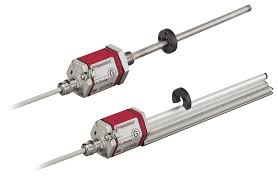
\includegraphics[width=0.3\linewidth]{img/sensorposicion}
	\caption{}
	\label{fig:sensorposicion}
\end{figure}


	$\cdot$Encóder incremental: Proporciona señales digitales proporcionales al movimiento. Necesita un punto de referencia para determinar la posición absoluta. Se usa en motores eléctricos y sistemas de control de movimiento.
	
	
\begin{figure} [h]
	\centering
	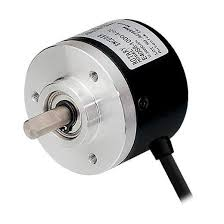
\includegraphics[width=0.3\linewidth]{img/encoderincremental}
	\caption{}
	\label{fig:encoderincremental}
\end{figure}

\newpage
	$\cdot$Encóder absoluto: Mide la posición absoluta sin necesidad de un punto de referencia. Se usa en aplicaciones donde la precisión y continuidad de la medición son críticas.


\begin{figure} [h]
	\centering
	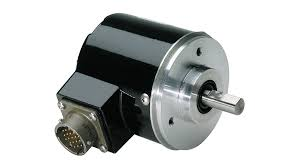
\includegraphics[width=0.3\linewidth]{img/encoderabsoluto}
	\caption{}
	\label{fig:encoderabsoluto}
\end{figure}


	$\cdot$Potenciómetro: Dispositivo resistivo que mide la posición angular o lineal mediante la variación de resistencia. Se emplea en controles de volumen y palancas de mando.
	
	
\begin{figure} [h]
	\centering
	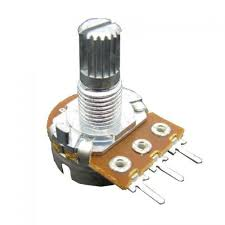
\includegraphics[width=0.3\linewidth]{img/potenciometro}
	\caption{}
	\label{fig:potenciometro}
\end{figure}


	$\cdot$LVDT (Transformador Diferencial Variable Lineal): Convierte el desplazamiento lineal en una señal eléctrica. Se usa en la medición de deformaciones y en máquinas industriales.


\begin{figure} [h]
	\centering
	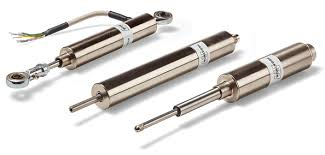
\includegraphics[width=0.3\linewidth]{img/lvdt}
	\caption{}
	\label{fig:lvdt}
\end{figure}

\newpage
	$\cdot$Résolver: Sensor electromagnético de posición angular utilizado en entornos de alta precisión y robustez. Común en aplicaciones aeroespaciales y de automatización industrial.
	
	
\begin{figure} [h]
	\centering
	\includegraphics[width=0.3\linewidth]{img/résolver}
	\caption{}
	\label{fig:resolver}
\end{figure}
	

\textbf{Sensores de Velocidad:}
	Determinan la rapidez con la que un objeto se desplaza. \cite{johnson2018sensores}.
	
	
\begin{figure} [h]
	\centering
	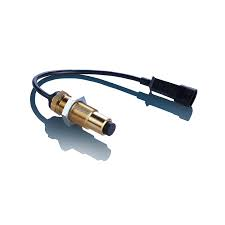
\includegraphics[width=0.3\linewidth]{img/sensorvelocidad}
	\caption{}
	\label{fig:sensorvelocidad}
\end{figure}


	$\cdot$Tacómetro: Mide la velocidad de giro de un eje o disco en revoluciones por minuto (RPM). Ampliamente usado en motores y sistemas de control de velocidad.


\begin{figure} [h]
	\centering
	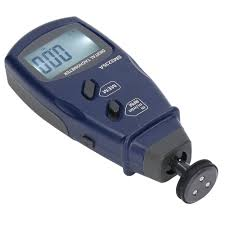
\includegraphics[width=0.3\linewidth]{img/tacometro}
	\caption{}
	\label{fig:tacometro}
\end{figure}

\newpage
	$\cdot$Sensor de efecto Hall: Utiliza el efecto Hall para medir la velocidad de un objeto en movimiento. Aplicado en sistemas de detección de velocidad en vehículos.


\begin{figure} [h]
	\centering
	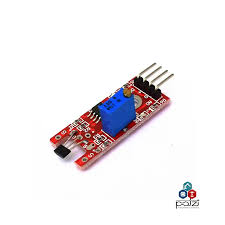
\includegraphics[width=0.3\linewidth]{img/sensorhall}
	\caption{}
	\label{fig:sensorhall}
\end{figure}


\textbf{Sensores de Aceleracion:}
	Detectan cambios en la velocidad de un objeto.

\begin{figure} [h]
	\centering
	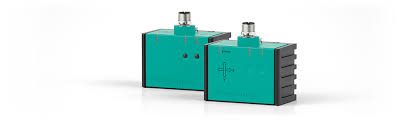
\includegraphics[width=0.3\linewidth]{img/sensoraceleracion}
	\caption{}
	\label{fig:sensoraceleracion}
\end{figure}


	$\cdot$Acelerómetros: Utilizados para detectar vibraciones y movimientos. Aplicaciones en teléfonos móviles, automóviles y dispositivos portátiles.


\begin{figure} [h]
	\centering
	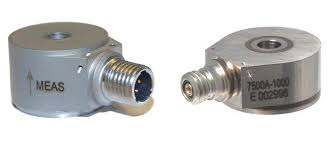
\includegraphics[width=0.3\linewidth]{img/acelerometrosensor}
	\caption{}
	\label{fig:acelerometrosensor}
\end{figure}


\textbf{Sensores de Fuerza:}
	Miden la cantidad de fuerza aplicada sobre un objeto.

\begin{figure} [h]
	\centering
	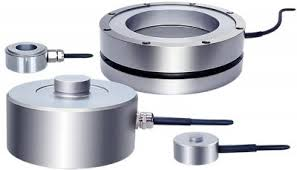
\includegraphics[width=0.3\linewidth]{img/sensorfuerza}
	\caption{}
	\label{fig:sensorfuerza}
\end{figure}

\newpage
	$\cdot$Galgas extensométricas: Detectan cambios en la resistencia eléctrica cuando un material se deforma. Usadas en básculas electrónicas y sistemas de monitoreo estructural.


\begin{figure} [h]
	\centering
	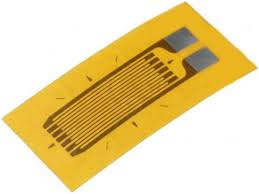
\includegraphics[width=0.3\linewidth]{img/galgasextensiometricas}
	\caption{}
	\label{fig:galgasextensiometricas}
\end{figure}


	$\cdot$Interruptores de efecto Hall: Se activan en presencia de un campo magnético. Utilizados en aplicaciones de detección de fuerza y proximidad.


\begin{figure} [h]
	\centering
	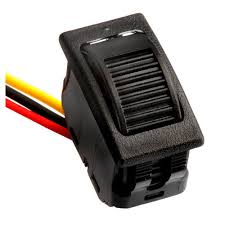
\includegraphics[width=0.3\linewidth]{img/interruptorhall}
	\caption{}
	\label{fig:interruptorhall}
\end{figure}


	$\cdot$Interruptores piezoeléctricos: Basados en materiales piezoeléctricos que generan una señal eléctrica bajo presión. Empleados en teclados táctiles y sensores de impacto.


\begin{figure} [h]
	\centering
	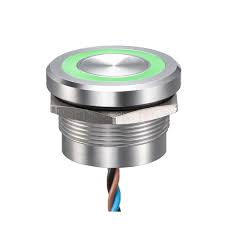
\includegraphics[width=0.3\linewidth]{img/interruptorpiezoelectrico}
	\caption{}
	\label{fig:interruptorpiezoelectrico}
\end{figure}

\newpage
\textbf{Sensores Externos} \cite{bryant2019robotics}.


\textbf{ Sensores de Contacto:}
	Se activan al entrar en contacto con un objeto.


\begin{figure} [h]
	\centering
	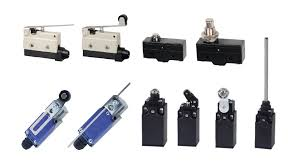
\includegraphics[width=0.3\linewidth]{img/sensorcontacto}
	\caption{}
	\label{fig:sensorcontacto}
\end{figure}


	$\cdot$Interruptores de límite: Detectan la presencia o ausencia de un objeto mecánicamente. Utilizados en automatización industrial y sistemas de seguridad.
	
	
\begin{figure} [h]
	\centering
	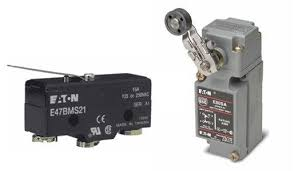
\includegraphics[width=0.3\linewidth]{img/interruptorlimite}
	\caption{}
	\label{fig:interruptorlimite}
\end{figure}
	
	
	$\cdot$Interruptores neumáticos: Funcionan con presión de aire para detectar la presencia de un objeto. Aplicados en sistemas neumáticos industriales.
	
	
\begin{figure} [h]
	\centering
	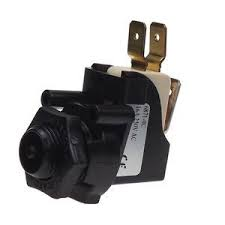
\includegraphics[width=0.3\linewidth]{img/interruptorneumaticp}
	\caption{}
	\label{fig:interruptorneumaticp}
\end{figure}
	
\newpage
	$\cdot$Sensores piezoeléctricos: Detectan vibraciones o impactos mediante materiales piezoeléctricos. Comunes en aplicaciones de monitoreo de estructuras y seguridad.


\begin{figure} [h]
	\centering
	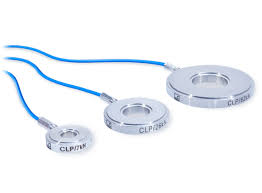
\includegraphics[width=0.3\linewidth]{img/sensorespiezoelectrico}
	\caption{}
	\label{fig:sensorespiezoelectrico}
\end{figure}


	$\cdot$Transductores de presión: Convierten la presión en una señal eléctrica. Usados en sistemas hidráulicos y neumáticos.
	
	
\begin{figure} [h]
	\centering
	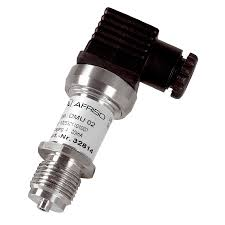
\includegraphics[width=0.3\linewidth]{img/transductordepresion}
	\caption{}
	\label{fig:transductordepresion}
\end{figure}
	
	
\textbf{Sensores sin Contacto:}
	Detectan objetos sin necesidad de contacto físico.
	
		
\begin{figure} [h]
	\centering
	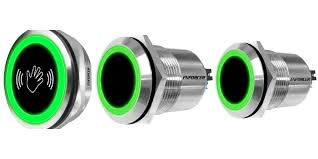
\includegraphics[width=0.3\linewidth]{img/sensoressincontacto}
	\caption{}
	\label{fig:sensoressincontacto}
\end{figure}
	
\newpage
	$\cdot$Sensores de proximidad: Detectan la presencia de un objeto cercano mediante diferentes tecnologías (inductiva, capacitiva, ultrasónica).
	
		
\begin{figure} [h]
	\centering
	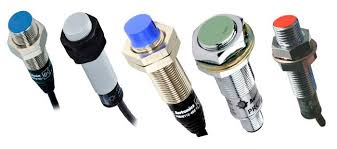
\includegraphics[width=0.3\linewidth]{img/sensoresdeproximidad}
	\caption{}
	\label{fig:sensoresdeproximidad}
\end{figure}


	$\cdot$Sensores de microondas: Emiten ondas de radio para detectar movimiento. Utilizados en sistemas de seguridad y detección de movimiento.
	
	
\begin{figure} [h]
	\centering
	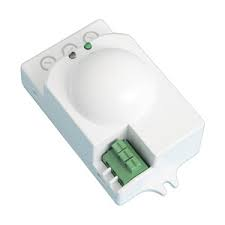
\includegraphics[width=0.3\linewidth]{img/sensormicroondas}
	\caption{}
	\label{fig:sensormicroondas}
\end{figure}
	
	
	$\cdot$Sensores ultrasónicos: Emplean ondas de sonido de alta frecuencia para medir distancias. Comunes en radares de estacionamiento y sistemas industriales.
	
	
\begin{figure} [h]
	\centering
	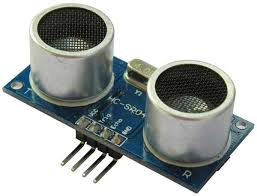
\includegraphics[width=0.3\linewidth]{img/sensorultrasonico}
	\caption{}
	\label{fig:sensorultrasonico}
\end{figure}
	
\newpage
	$\cdot$Sensores láser: Usan haces de luz láser para medir distancias con precisión. Aplicados en topografía y control de calidad.
	
	
\begin{figure} [h]
	\centering
	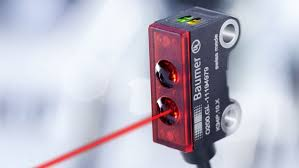
\includegraphics[width=0.3\linewidth]{img/sensorlaser}
	\caption{}
	\label{fig:sensorlaser}
\end{figure}

	$\cdot$Sensores de visión: Cámaras avanzadas utilizadas para reconocimiento de objetos y seguimiento visual. Aplicados en robótica, automatización y control de calidad.
	
	
\begin{figure} [h]
	\centering
	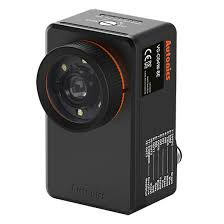
\includegraphics[width=0.3\linewidth]{img/sensorvision}
	\caption{}
	\label{fig:sensorvision}
\end{figure}
\newpage

